\documentclass{article}

% Package Declarations
\usepackage{arxiv}
\usepackage[utf8]{inputenc} % allow utf-8 input
\usepackage[T1]{fontenc}    % use 8-bit T1 fonts
\usepackage{hyperref}       % hyperlinks
\usepackage{url}            % simple URL typesetting
\usepackage{booktabs}       % professional-quality tables
\usepackage{amsfonts}       % blackboard math symbols
\usepackage{nicefrac}       % compact symbols for 1/2, etc.
\usepackage{microtype}      % microtypography
\usepackage{lipsum}         % Lorem Ipsum fill text
\usepackage{multicol}       % Support for Multi columns for tables
\usepackage{multirow}       % Support for Multi rows fot tables
\usepackage{mathtools}      % Advanced mathtools
\usepackage{caption}        % Advanced caption configuration
\usepackage{amsmath}        % Math package for equations       
\usepackage{titlesec}       % Title section
\usepackage{graphicx}       % For adding labels to parts of the equation
\usepackage{stackrel}       % For adding labels to parts of the equation
\usepackage[ruled,vlined]{algorithm2e}  % For Algorithms
\usepackage{algorithm}
\usepackage{algpseudocode}


% Theme Configurations

% Set section depth to 4
% \setcounter{secnumdepth}{4}

% \titleformat{\paragraph}
% {\normalfont\normalsize\bfseries}{\theparagraph}{1em}{}
% \titlespacing*{\paragraph}
% {0pt}{3.25ex plus 1ex minus .2ex}{1.5ex plus .2ex}

% Add padding to text below table
\captionsetup[table]{skip=10pt}

% Configure hat tex
\let\oldhat\hat
\renewcommand{\hat}[1]{\oldhat{\mathbf{#1}}}

% Block comment - \comment{
% multiline
% }
\newcommand{\comment}[1]{}

% Document Start

\title{Differentiable Learning by means of Neural Network Pruning}

\author{
  Prathyush S Parvatharaju$\ ^{1}$\\
%   \thanks{Use footnote for providing further
%     information about author (webpage, alternative
%     address)---\emph{not} for acknowledging funding agencies.} \\
  Department of Data Science\\
  Worcester Polytechnic University\\
  Worcester, MA 01609 \\
  \texttt{psparvatharaju@wpi.edu} \\
  %% examples of more authors
   \And
 Shreesha Narasimha Murthy$\ ^{2}$ \\
  Department of Data Science\\
  Worcester Polytechnic University\\
  Worcester, MA 01609 \\
  \texttt{snarasimhamurthy@wpi.edu} \\
}

\begin{document}
\maketitle



\begin{abstract}
The idea of linear flow i.e, each node in a layer is connected to a certain weight $\hat{W_{ij}}$ to every other node in the following layer, for the deep neural network is limiting in the sense of the way we, humans think. It is a constraint for DNN as they process data and emulate relationships in higher dimensions. By replacing the linear flow with a gradient-based decision process combined with skip connections give the ability for the network to develop much deeper constructs from minimal data. We propose a novel idea of extending the capabilities of previously used short-circuits as differentiable functions, essentially solving “What to feed?”. To tackle the problem, “When to stop?” we propose an algorithm for early stopping criterion based on Information Transfer derived from differentiable short-circuits. 

In our experiments, we show that the increase in weighted representation capability of the network results in achieving better accuracy in fewer iterations compared to the standard architecture. We also demonstrate that with 10\% of the previous parameters, the architecture achieves similar results and builds better representations with minimal data compared to a standard architecture. In the end, we demonstrate differentiable short-circuit's ability to visualize the relevant features for a given layer as it learns to drop common features among different classes and this reduces class ambiguity and thereby increasing the confidence score of a class.
\end{abstract}


% keywords can be removed
\keywords{Differentiable Learning \and Pruning \and Neural Architecture Search}


\section{Introduction}
The ability to recognize patterns and develop strong relations among them has made neural networks supersede state of the art machine learning techniques. The depth of representations is of central importance for many visual recognition tasks. Right from Alex Net \cite{Krizhevsky2012ImageNetCW} up until ResNet \cite{He2016DeepRL} the flow of data followed a linear fashion i.e the data flow from one layer to the next layer and so on. ResNet brought in innovation by creating \emph{"Short Circuits"} - there exists a skip connection where, as usual, data is fed to the next layer and in certain circumstances, it is fed to the layer after its immediate next. This paved way to train deep-networks as it increased the representational capability of the network by overcoming issues such as vanishing / exploding gradients \cite{Bengio1994LearningLD, Glorot2010UnderstandingTD}. In our work we set out a goal to explore the \emph{"representational capability"} and its effects on the performance of the network. This led to the question - "What to feed?".

ResNet brings in short circuits between residual components and the number of skip connections is restricted. We propose \emph{"Global Short Circuit"}(GSC), a neural architecture to investigate the behavior of short circuits by revoking the restriction and providing skip connections from one layer to every other layer. Thereby enhancing the representational capability of the network and therefore yields better accuracy in fewer iterations compared to the standard architecture (See section \ref{sssec:ffn}). However, this modification results in a large network, due to which we observer an exponential increase in the trainable parameters, rendering the network unscalable. As a solution, we propose an enhanced version of GSC i.e, \emph{" Differentiable Short Circuit"}(DSC) - a novel neural architecture to help network scale by pruning unwanted connections over time.

To tackle the issue of \emph{"When to stop"}?, we propose \emph{Information Transfer Rate}. It is a measure of the amount of flow of data from one layer to another. Keeping track of the variance of \emph{information transfer rate} over iterations, based on a certain threshold,  we formulate a stopping criterion.

\section{Differentiable Learning}
\label{sec:headings}

Neural networks are differentiable by design. The standard neural architecture (Section\ref{sssec:ffn}) is static and does not change over time. However, learning changes over time. To adapt the neural architecture to the dynamics of learning, there have been efforts towards an automated way of finding the best architecture for the given data i.e, Neural Architecture Search (NAS) \cite{Zoph2016NeuralAS}. The recent advent of DARTS \cite{Liu2019DARTSDA} a differentiable NAS, suggests that a learning-based adaptive architecture performs better compared to a static architecture. To understand the nature of selection criteria, we have to learn the connectivity amongst individual neurons. For instance, given $N$ layers, to identify the optimal data paths, we can use brute-force and try out $n(n-1)$ combinations of connections. However, as the depth of the network increases, the search space increases exponentially, and training each configuration becomes a tedious and time-consuming process. Gradient descent \cite{ruder2016overview} - a first-order iterative search space optimization algorithm that finds a local minimum of a differentiable function can be used to find the optimal skip connections. Initially, we describe a standard feed-forward neural network and later propose, Global short circuit (GSC) and Differentiable Short Circuit (DSC) neural architectures.

\subsection{Feed Forward Neural Network}
\label{sssec:ffn}
Multilayer perceptron trained using back-propagation \cite{Rumelhart1986LearningIR}, a supervised learning algorithm is capable of approximating solutions for complex problems. Acting as a universal approximator, the architecture has a linear flow; i.e, a layer takes the output of the immediate previous layer alone as its input. Also known as a densely connected layer, it provides learning features from all the combinations of the features of the previous layer. With a linear increase in the number of connections (based on the nodes in the layer) the architecture is scalable and is time-efficient. $\hat{Z}$ in Equation \ref{eq:affine_transformation} is the result of an affine transformation and is capable of learning an offset ($\hat{b}$) and a rate of correlation ($\hat{W}$) that fits the given input.

\begin{equation}
\label{eq:affine_transformation}
\begin{aligned}
\hat{Z} &= Input \cdot \hat{W} + \hat{b}&\\
\end{aligned}
\end{equation}

This type of transformation can only learn linear relationships. In order to learn any non-linearity, a squashing non-linear transformation - sigmoid $(\sigma)$ \cite{Han1995TheIO} is applied to the output of each node. Termed as an activation function, it results in a probability as it restricts the range of the output between 0 and 1.

\begin{equation}
\label{eq:sigmoid_activation}
\begin{aligned}
\sigma(z) &= \frac{1}{1+e^{-z}} \;\;\;\;\;\;  x\in\mathbb{R}, 0<\sigma(x)<1
\end{aligned}
\end{equation}

Figure \ref{fig:SimpleFFN.png} represents a standard feed-forward architecture and equation \ref{eq:ffn_math_representation} is the mathematical formulation of the network. Each node in one layer is connected to a certain weight $\hat{W_{ij}}$ to every node in the following layer. 

\noindent\begin{minipage}{.45\textwidth}
   \centering
   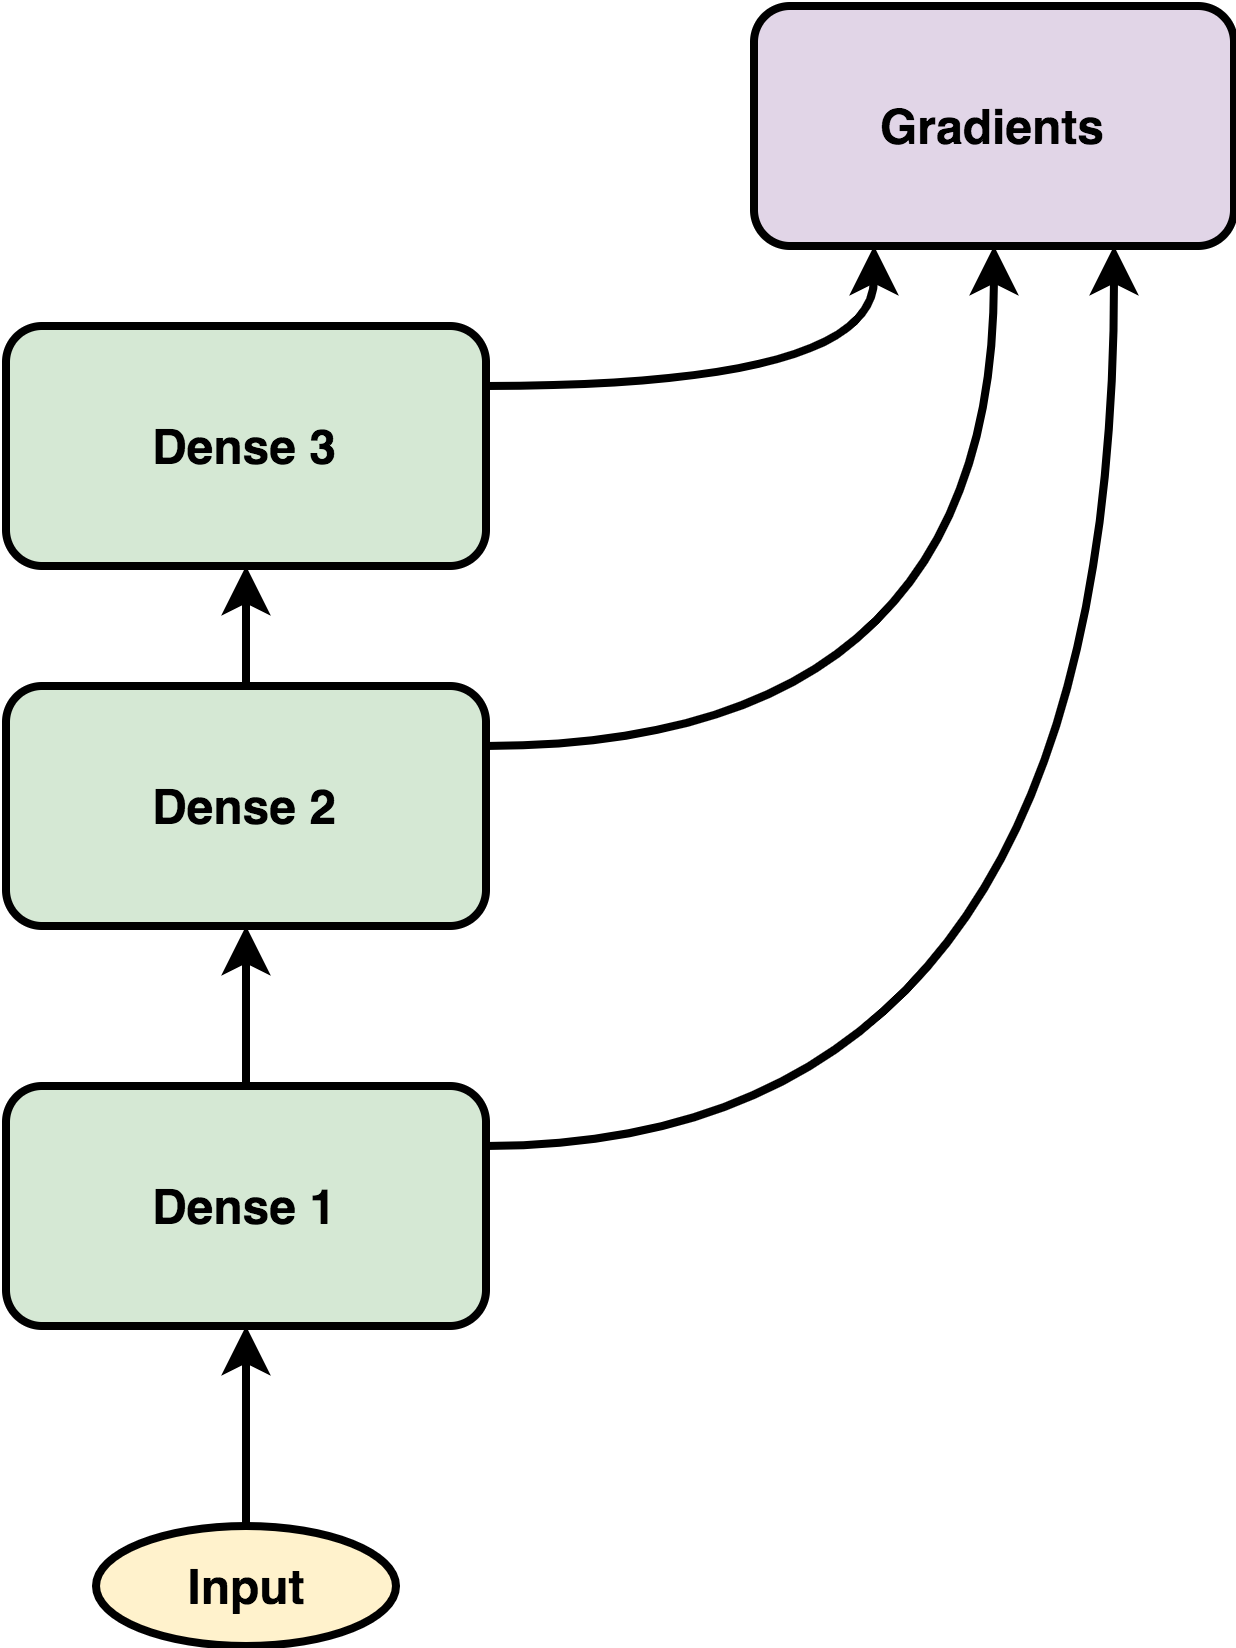
\includegraphics[scale=0.09]{SimpleFFN.png}
   \captionof{figure}{Feed Forward Network}
   \label{fig:SimpleFFN.png}
\end{minipage}
\begin{minipage}{.45\textwidth}
\begin{equation}
\label{eq:ffn_math_representation}
\begin{aligned}
   Dense_{1} &= \sigma(Input \cdot \hat{W}_{1} + \hat{b}_{1}) &\\
   Dense_{2} &= \sigma(Dense_{1} \cdot \hat{W}_{2} + \hat{b}_{2}) &\\
   Dense_{3} &= \sigma(Dense_{2} \cdot \hat{W}_{3} + \hat{b}_{3}) 
\end{aligned}
\end{equation}
\end{minipage}

For the previously mentioned standard network, the number of trainable parameters for a given layer is a function of the layer's weight, bias, and input. For a given network, the same is represented as, 

\begin{equation}
\label{eq:ffn_params}
\begin{aligned}
Params &= \sum_{n=1}^{N}
\underbrace{(l_{n-1}\rule[-12pt]{0pt}{5pt}}_{\mbox{input}}
*\underbrace{l_{n})\rule[-12pt]{0pt}{5pt}}_{\mbox{weights}}
+\underbrace{l_{n}\rule[-12pt]{0pt}{5pt}}_{\mbox{bias}} &\\
\text{where}~N &= \text{Number of layers} \\
l_{n} &= \text{Number of nodes in the layer}\\
\end{aligned}
\end{equation}

For a 3 layer network with node configurations [100,50,10] and 784 input features, using equation \ref{eq:ffn_params} we arrive at 83,550 trainable parameters


\subsection{Global Short Circuit (GSC)}
This work proposes \emph{"Global Short Circuit"} neural architecture to explore the impact of skip connections on the representational capabilities of the network. There exists a connection from every layer to every succeeding layer in the network. Some of the possible ways of merging layers are explored in DenseNet\cite{Li2018DenselyCC} and ResNet\cite{He2016DeepRL}. In ResNet weighted feature maps are merged using $max$ or $sum$. DenseNet merges features using a concatenation operation. We define a merge operation similar to DenseNet's $concat$ . However, this type of merging has an issue when it comes to Convolutional layers, where there is a requirement to merge feature maps of different shapes, unlike feed-forward layers. As a solution, we use downsampling/padding operators to get identical shapes for the merge operation. Figure \ref{fig:GSC.png} shows the standard architecture defined in section \ref{sssec:ffn} having connections from one layer to the subsequent layers, merged using concat operation. The difference in the connections between the layers is relative to the number of gradient operations required for the respective layer. Equation \ref{eq:gsc_math_representation} provides mathematical representation of the architecture.

\noindent\begin{minipage}{.45\textwidth}
   \centering
   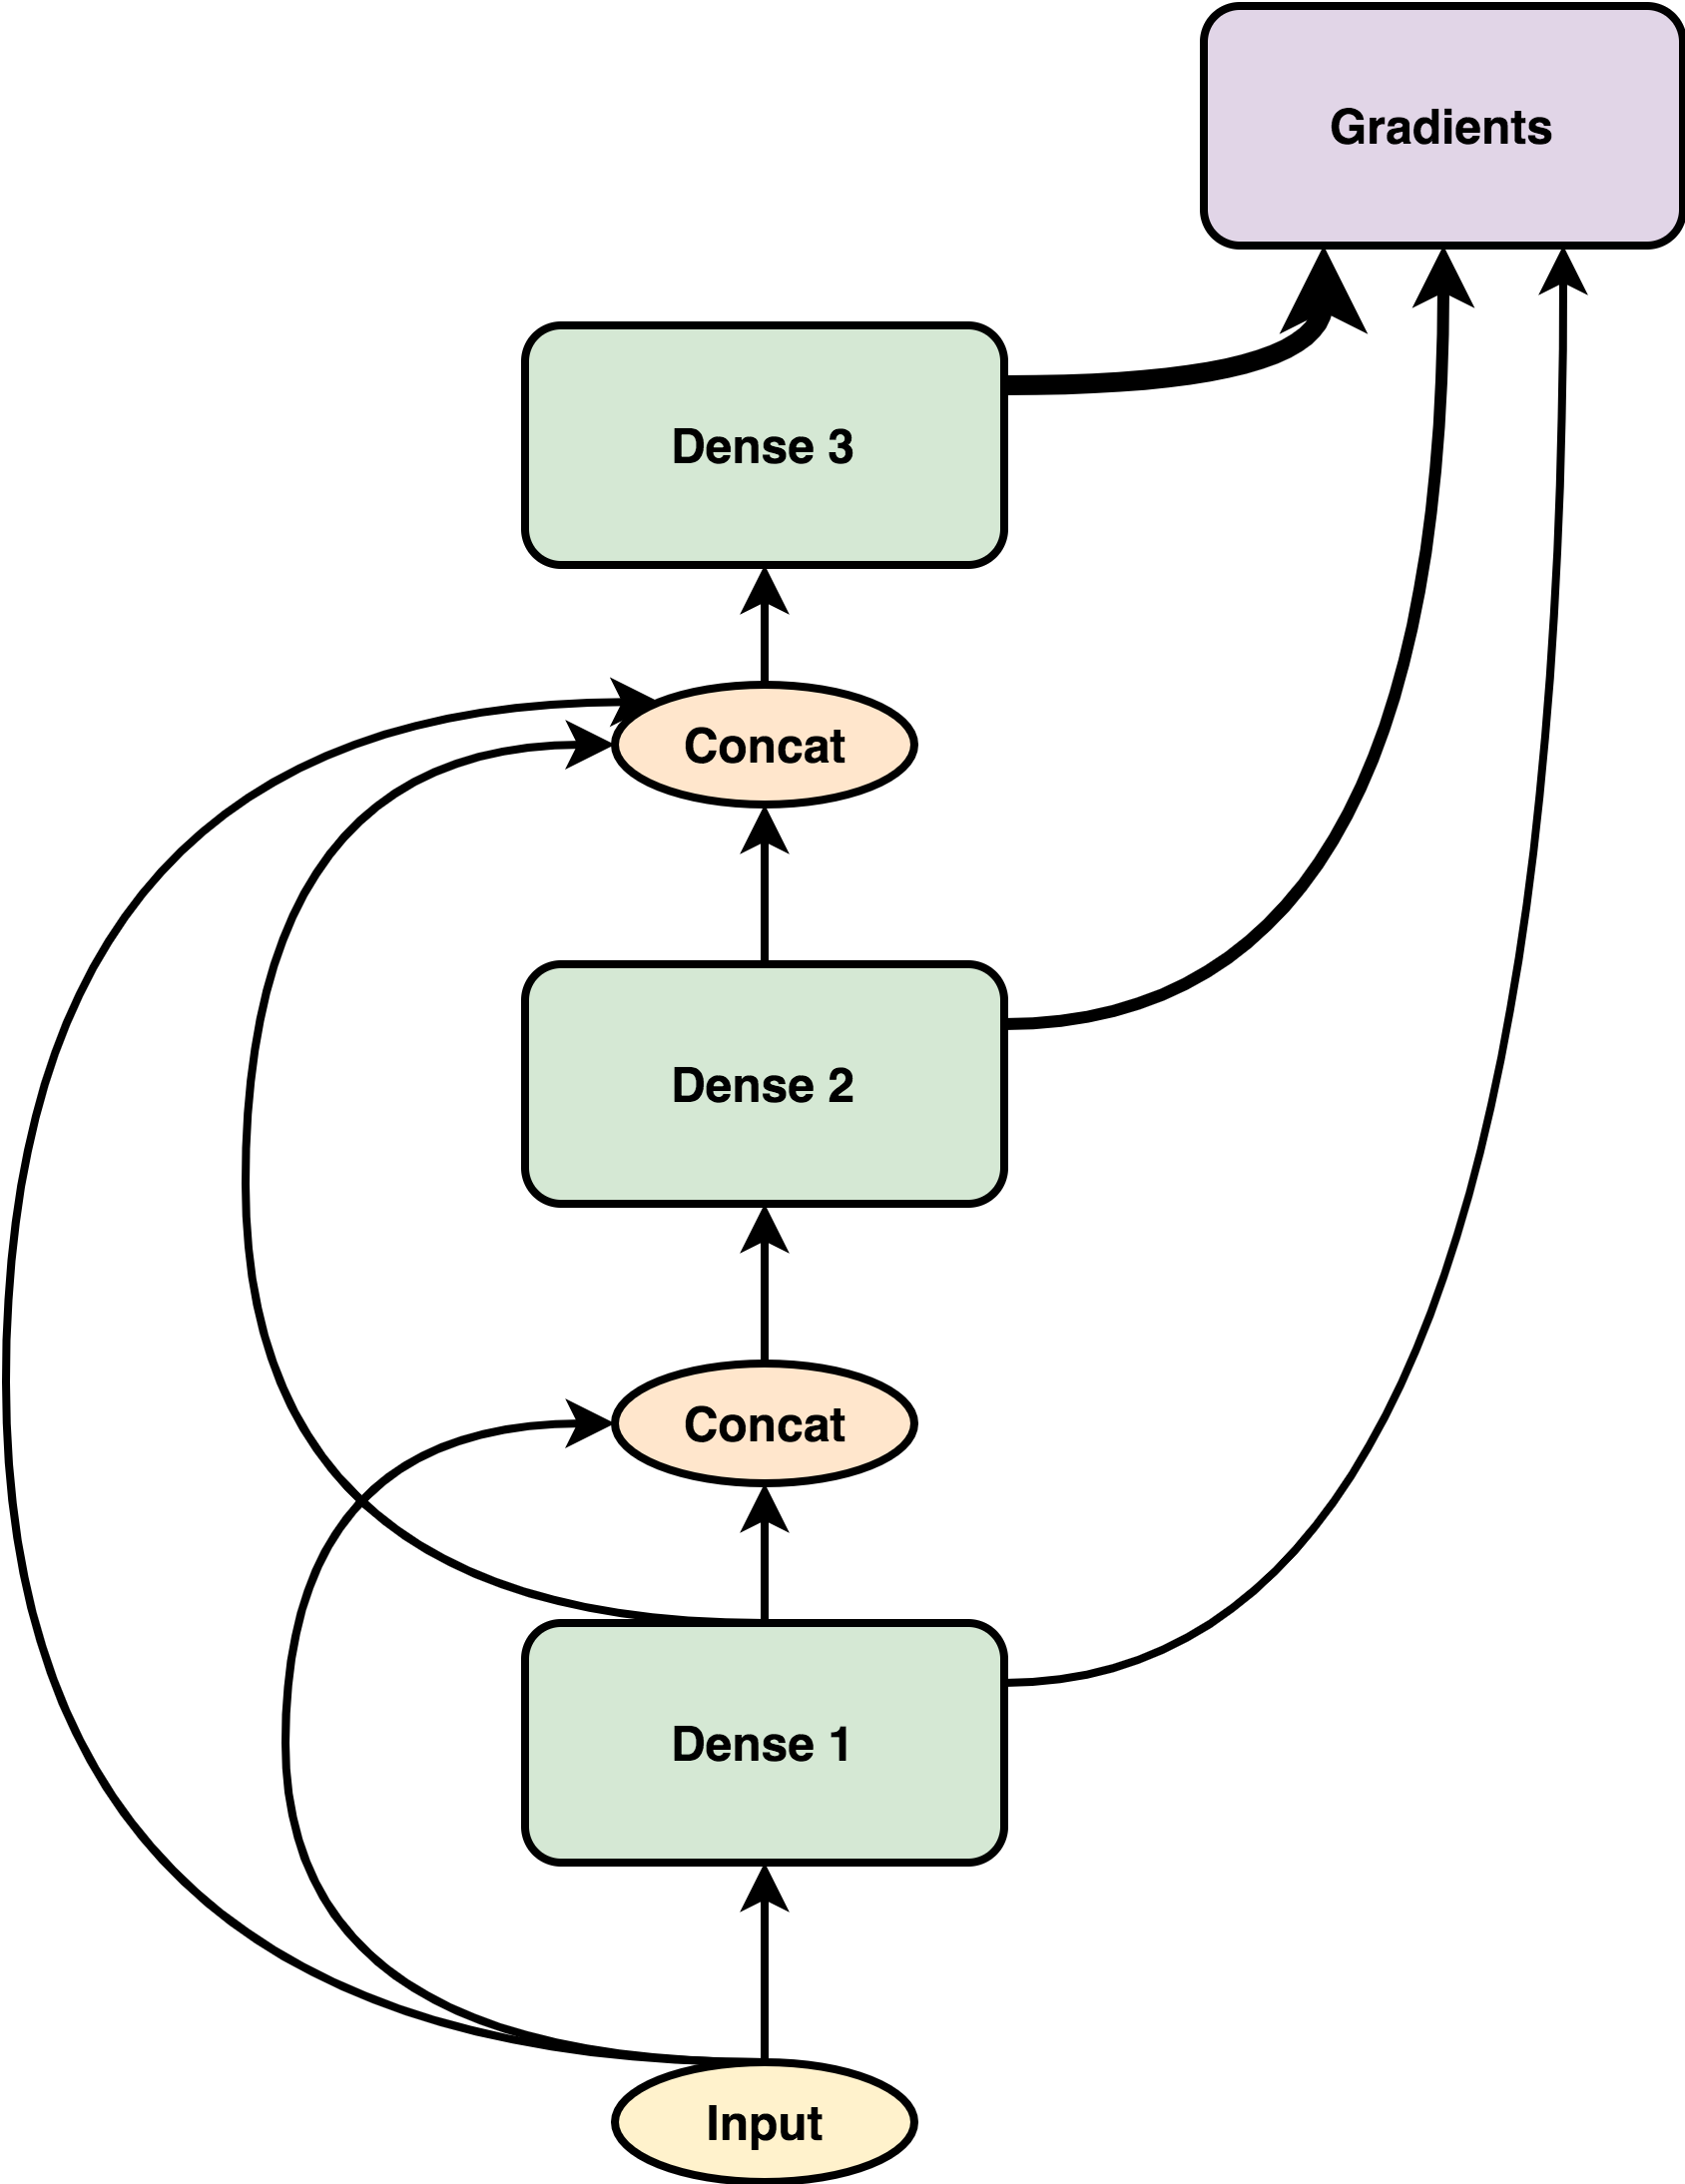
\includegraphics[scale=0.09]{GSC.png}
   \captionof{figure}{Global Short Circuit}
   \label{fig:GSC.png}
\end{minipage}
\begin{minipage}{.45\textwidth}
\begin{equation}
\label{eq:gsc_math_representation}
\begin{aligned}
       Dense_{1} &= \sigma(Input \cdot \hat{W}_{1} + \hat{b}_{1}) &\\
       Dense_{2} &= \sigma([Input \oplus Dense_{1}] \cdot \hat{W}_{2} + \hat{b}_{2}) &\\
       Dense_{3} &= \sigma([Input \oplus Dense_{1} \oplus Dense_{2}] \cdot \hat{W}_{3} + \hat{b}_{3}) 
\end{aligned}
\end{equation}
\end{minipage}

Experiments show that GSC achieves better accuracy compared to standard architecture on various datasets (See section \ref{sec:experiments}). This is due to increased representational capacity of the network. A layer \emph{n} in the network now has access to every \emph{n-1} previous outputs. This change paves way to create much deeper constructs and complex relationships among the layers. To advocate that our proposed method - GSC creates much deeper constructs than the standard architecture, the class confidences of the predictions are measured. Confidence score is unique for each class and the use of \emph{Softmax} function restricts the score between 0 and 1. At the end of each epoch, mean of class confidence scores are calculated across a large unseen test set. This measure speaks for the trust in the prediction. Among the variable factors of the measure, the rate of increase and the actual value are vital for the analysis. MNIST \cite{LeCun1998GradientbasedLA}, Fashion-MNIST \cite{Xiao2017FashionMNISTAN}, CIFAR-10 datasets \cite{Krizhevsky2009LearningML} are chosen to account for the variability in the pattern complexity. The training samples are restricted to 10\% of the whole, while still maintaining a large test sample to test the described hypothesis. Figure \ref{fig:cscore_100p_model.png} shows the performance when the node level configurations across standard and GSC are the same. GSC has 30\% more trainable parameters due to merge operation. To rule out the difference in the trainable parameters as a reason for achieving high confidence scores, we create 10p architectures. Here, the node level configurations across the models varies but the number of trainable parameters are kept constant across all architectures. The performance of 10p architectures are shown in Figure \ref{fig:cscore_10p_model.png}.  

\noindent\begin{minipage}{.5\textwidth}
   \centering
   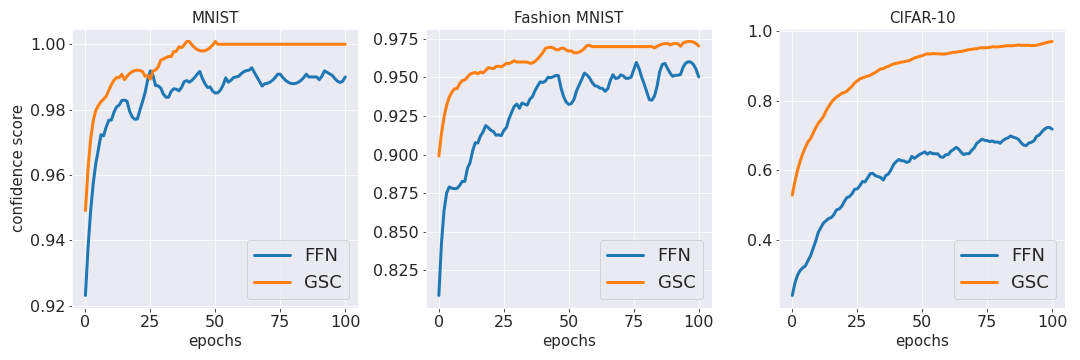
\includegraphics[scale=0.2]{paper/cscore_100p_param.png}
   \captionof{figure}{10p Data, 100p Model}
   \label{fig:cscore_100p_model.png}
   \centering
   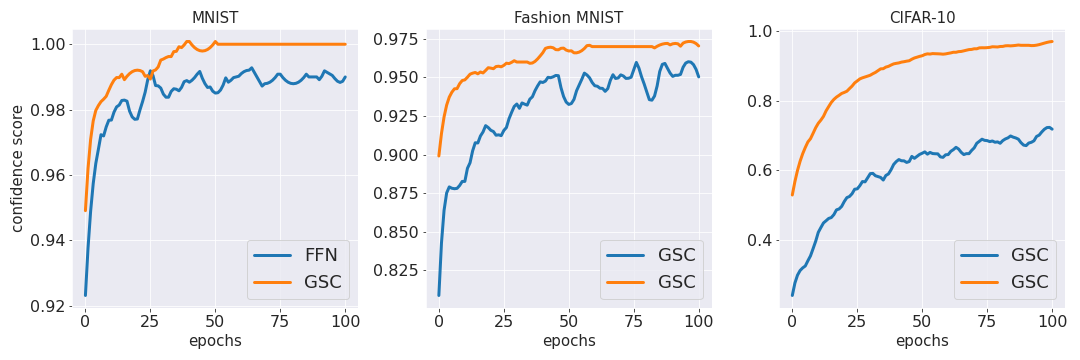
\includegraphics[scale=0.2]{paper/cscore_10p_param.png}
   \captionof{figure}{10p Data, 10p Model}
   \label{fig:cscore_10p_model.png}
\end{minipage}
\begin{minipage}{.4\textwidth}
In figure \ref{fig:cscore_100p_model.png} the difference in the confidence scores of MNIST among standard and GSC is negligible. This is due to the lack of complex patterns across classes in the dataset. There is a marginal difference in the score in Fashion MNIST and a distinct difference in CIFAR-10. CIFAR-10 comprises of 10 classes of real-world complex object patterns and GSC neural architecture enables the model to create much deeper constructs compared to the standard architecture. We notice a similar behavior in the confidence measure across 10p architectures where the number of trainable parameters across the networks is kept constant.
\end{minipage}


However, GSC suffers from an exponential increase in connections resulting in delayed training time. A rise in the number of stacked layers is noticed with the increase in the complexity of the network in terms of depth and is not a scalable solution. Compared to the standard architecture, GSC has a considerable expansion in the number of training parameters. This is due to the effect of merge operations of previous $n-1$ layers for every $n$ layer.

\begin{equation}
\label{eq:gsc_params}
\begin{aligned}
Params &= \sum_{n=1}^{N}\left[
\underbrace{(\sum_{i=0}^{n}l_{i}\rule[-12pt]{0pt}{5pt}}_{\mbox{merged inputs}}
*\underbrace{l_{n})\rule[-12pt]{0pt}{5pt}}_{\mbox{weights}}
+\underbrace{l_{n}\rule[-12pt]{0pt}{5pt}}_{\mbox{bias}}\right] &\\
\text{where}~N &= \text{Number of layers} \\
l_{n} &= \text{Number of nodes in the layer}\\
\end{aligned}
\end{equation}

For the aforementioned 3 layer network, an exponential increase of 30\% i.e, 122,750 parameters has to be trained.

\subsection{Differentiable Short Circuit (DSC}
\label{sec:dsc}
Finally, we propose a Differentiable Short Circuit (DSC) neural architecture to counter the effect of the exponential increase in training parameters due to merge operation. It is done so by expressing the connection between layers as a weighted sigmoid gate. For a connection, we introduce connection weight $\hat{C}$, a trainable parameter whose suitable values are found using $\frac{\partial loss}{\partial \hat{C}}$. A change in the value of the connection weight affects the loss. Based on this, we use the gradient descent algorithm to obtain optimum values for connection weight. The direction and magnitude of the weight affect the performance of the network, by introducing undesired changes in the architecture. 

To check these effects, a transformation function that is capable of restricting the direction and magnitude of the weight in a specified range is used. Neural arithmetic logic unit \cite{Trask2018NeuralAL} propose a layer whose transformation matrix $\hat{W}$ consists just of -1's, 0's and 1's. To prevent the layer from changing the scale of the representation of the numbers when mapping the input to the output, a squashing non-linearity ($\sigma$) is applied on just the weights, $\hat{W}$.  Hence, the sigmoid function, defined in equation \ref{eq:sigmoid_activation}, is applied on $\hat{C}$. Along with forcing the range of output to be in a specific interval, it also helps in preserving the direction of the input. 

With the use of weighted sigmoid gates, gives the network a chance to distinguish between essential and redundant data pathways. Based on a certain threshold, we propose a pruning algorithm which over time, learns to delete redundant connections. Each value in the weight of a layer is optimized based on the conditional dependence among others. Hence it is essential to start with all possible connections so that the network can develop stronger constructs before the prune operation. Pruning introduces sparsity in the network, decreasing training time exponentially. The proposed solution has the advantages of GSC without adding a major overhead to the training time. Figure \ref{fig:DSC.png} shows the use of connection weights, applied to the output of concat operation, essentially keeping the connection in check before it is fed to the next layer. The difference in the representation of connections between various blocks and the gradient operation shows the number of gradient computations required for the layer or the operation. Equation \ref{eq:dsc_math_representation} provides mathematical representation of the network.

\noindent\begin{minipage}{.45\textwidth}
   \centering
   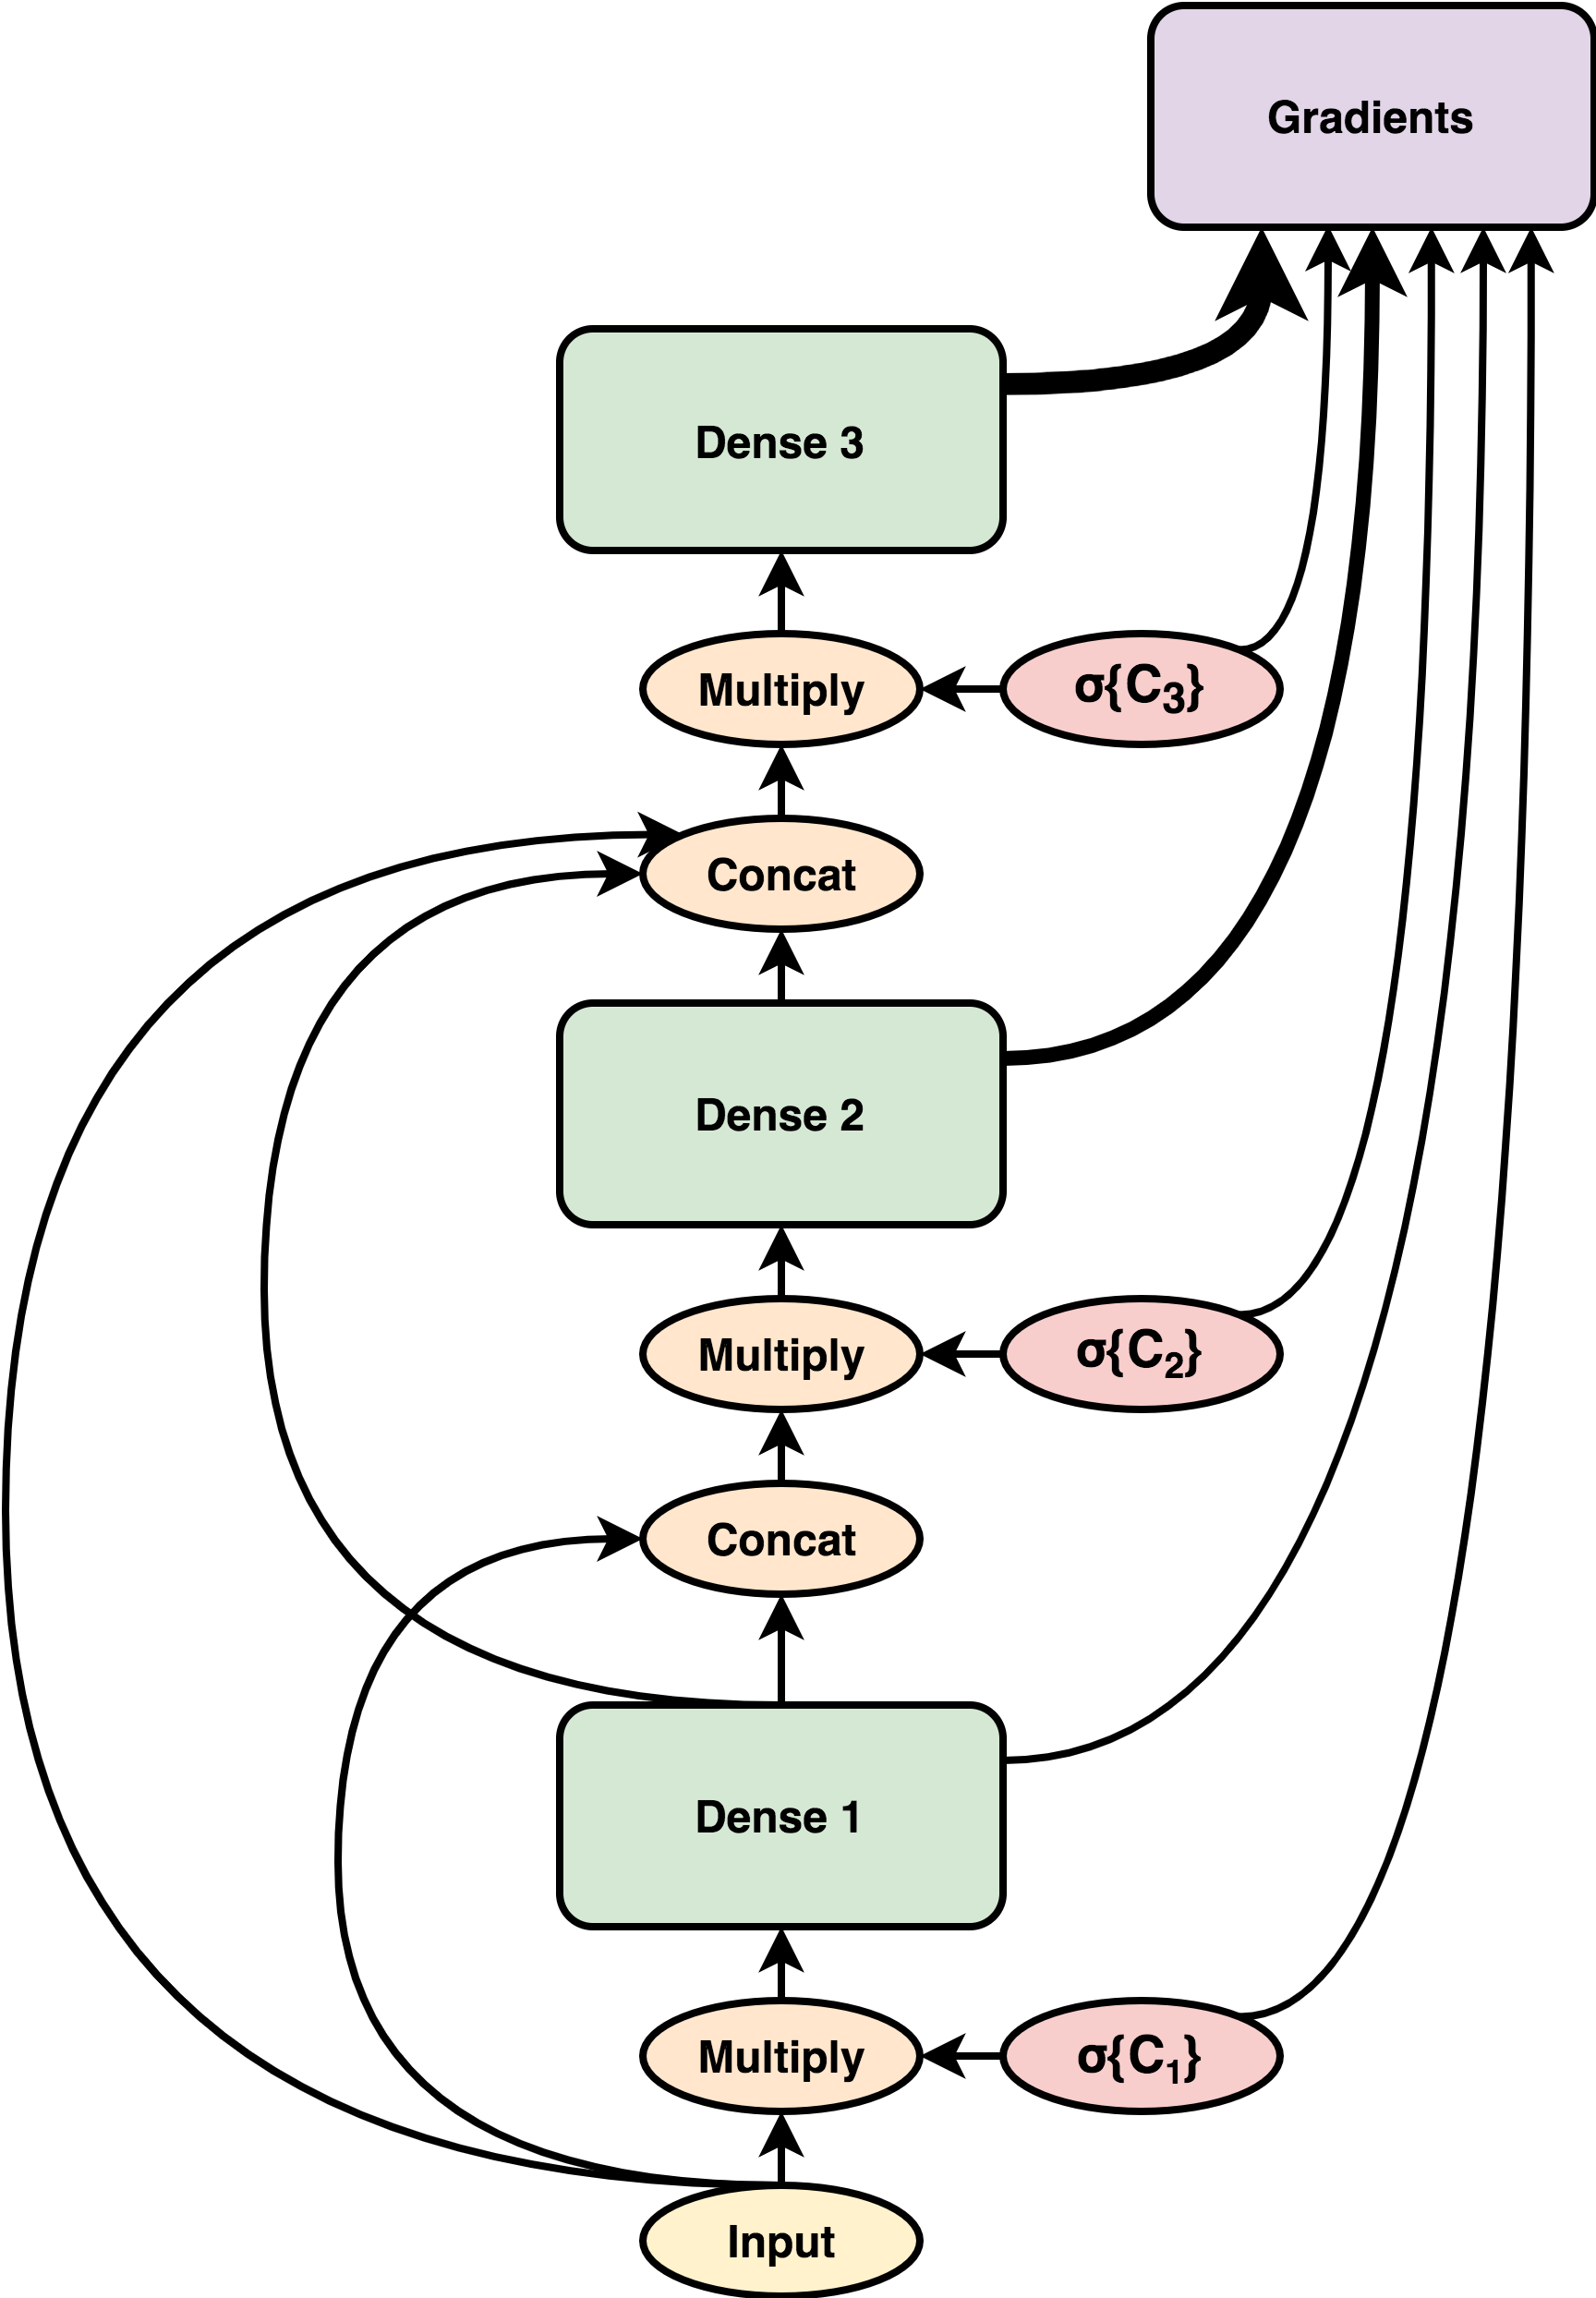
\includegraphics[scale=0.09]{DSC.png}
   \captionof{figure}{Differentiable Short Circuit}
   \label{fig:DSC.png}
\end{minipage}
\begin{minipage}{.45\textwidth}
\begin{equation}
\label{eq:dsc_math_representation}
\begin{aligned}
   Dense_{1} &= \sigma((\sigma(\hat{C}_{1}) \cdot Input) \cdot \hat{W}_{1} + \hat{b}_{1}) &\\
   Dense_{2} &= \sigma((\sigma(\hat{C}_{2}) \cdot [Input \oplus Dense_{1}]) \cdot \hat{W}_{2} + \hat{b}_{2}) &\\
   Dense_{3} &= \sigma((\sigma(\hat{C}_{3}) \cdot [Input \oplus Dense_{1} \oplus Dense_{2}]) \cdot \hat{W}_{3} + \hat{b}_{3}) 
\end{aligned}
\end{equation}
\end{minipage}

For DSC, we notice a slight increase in trainable parameters compared to GSC's equation \ref{eq:gsc_params} due to the use \emph{weighted gates}. There exists a trainable gate for every connection. The number of parameters for connections is defined by $\sum_{i=0}^{n}l_{i}$, where $l_{i}$ represents the number of incoming connections for a layer. As a result, for the network structure defined in the standard architecture, the number of trainable parameters are 124,418, a rise of 1.3\% over GSC and 32\% over the standard architecture. However, due to the use of pruning, the number of parameters decreases significantly over time, reducing training overhead.

\begin{equation}
\label{eq:dsc_params}
\begin{aligned}
Params &= \sum_{n=1}^{m}\left[
\underbrace{(\sum_{i=0}^{n}l_{i}\rule[-12pt]{0pt}{5pt}}_{\mbox{merged inputs}}
*\underbrace{l_{n})\rule[-12pt]{0pt}{5pt}}_{\mbox{weights}}
+\underbrace{l_{n}\rule[-12pt]{0pt}{5pt}}_{\mbox{bias}}
+\underbrace{\sum_{i=0}^{n}l_{i}\rule[-12pt]{0pt}{5pt}}_{\mbox{connection weights}}\right] &\\
\\
\text{where}~N &= \text{Number of layers} \\
l_{n} &= \text{Number of nodes in the layer}\\
\end{aligned}
\end{equation}
The benefit of having trainable gates are of two folds,

1. By keeping track of the variance of $\sigma{(\hat{C})}$ over time has proven to be useful in designing a stopping criterion, elucidated in section \ref{sub:InfoTransfer}. The connection weights associated with the input layer to every other layer can be expressed as a saliency score for a pixel in the input. Using these, we visualize the network's behavior in selecting the required features and discarding the rest. (Details in Section \ref{subsec:understanding_connection_weights})

2. Since the output of the gates is probabilistic, we use a binary threshold function to transform continuous values into a binary mask. The mask is then used to prune unwanted skip connections. Section \ref{sec:Pruning} describes the pruning methodology in detail.

\par
\bigskip

\par
\bigskip

\par
\bigskip

\subsubsection{Information Transfer Rate}
\label{sub:InfoTransfer}
We propose \emph{Information transfer rate} (itr) as a percentage measure of the data flow from one layer to the next. The weighted gated connections having sigmoid activation translates to a scaling operation. Each output is scaled based on its significance before the same is fed to the next layer. The scaling transformation is also applied to skip connections as shown in figure \ref{fig:DSC.png}. Equation \ref{eq:itr} describes the rate of information transfer from one layer to the next. 

    \begin{equation}
    \label{eq:itr}
    \begin{aligned}
    itr_{layer} &=\frac{\sum_{c=1}^{N}\hat{W}_{c}}{|\hat{W}_{c}|}, \\
    \\
    \text{where}~N &= \text{Number of nodes,} \\
    \hat{W}_{c} &= \text{Connection weight}\\
    |\hat{W}_{c}| &= \text{Length of connection weight}\\
\end{aligned}
\end{equation}

To calculate the information transfer of the network, based on the number of layers and their respective information transfer rates, we propose Equation \ref{eq:itr_mean}.  It is a conditional mean of ${itr_{layers}}$. There are no \emph{recurrent} associations and connections are always \emph{unidirectional}. Figure \ref{fig:sample_info_transfer} represents ${itr_{layer}}$ in a matrix format. The first column represents \emph{"from"} and the first row shows \emph{"to"} relations. Ex: From $Dense\>1$ to $Dense\>3$ the gated data flow is measured at 26\%.


\noindent\begin{minipage}{.45\textwidth}
   \centering
   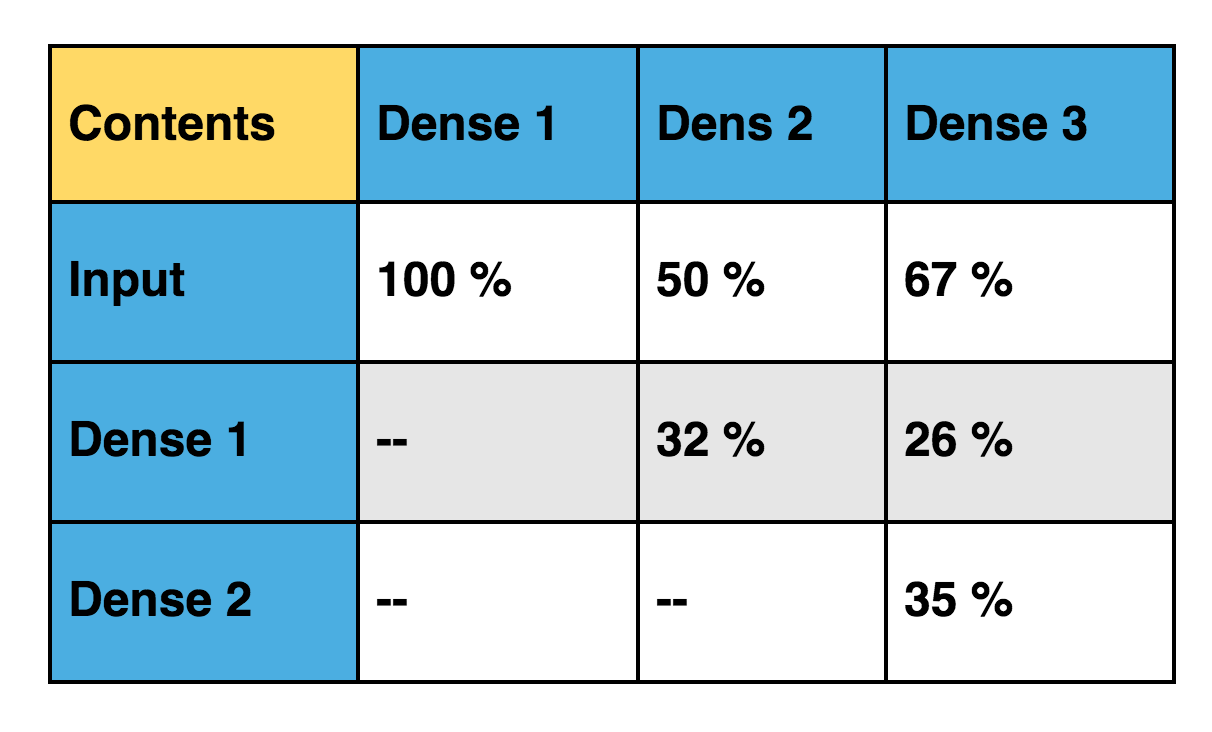
\includegraphics[scale=0.13]{paper/SampleTable.png}
   \captionof{figure}{Sample Information Transfer}
   \label{fig:sample_info_transfer}
\end{minipage}
\begin{minipage}{.45\textwidth}
\begin{equation}
\label{eq:itr_mean}
\begin{aligned}
itr_{network} &= \frac{\sum_{i=0}^{n-1}\sum_{j=1}^{n} 
\begin{cases}
  itr_{ij}, & \text{if}\ i<j \\
  0, & \text{otherwise}
\end{cases}}{\frac{n(n+1)}{2}}\\
\text{where}~n &= \text{Number of layers} \\
\end{aligned}
\end{equation}
\end{minipage}


Figure \ref{fig:iv.png} shows that over time, the number of features picked by the network saturates. On close observation, the saturation point of the $itr_{network}$ metric is similar to the saturation point of the accuracy function. MNIST and Fashion MNIST datasets are relatively easy datasets compared to CIFAR-10 and the saturation point of the metric can be used as an early-stopping criterion. In CIFAR-10, the metric changes over time and so does the accuracy and hence it does not meet the early exit criterion.

\begin{figure}[H]
\centering
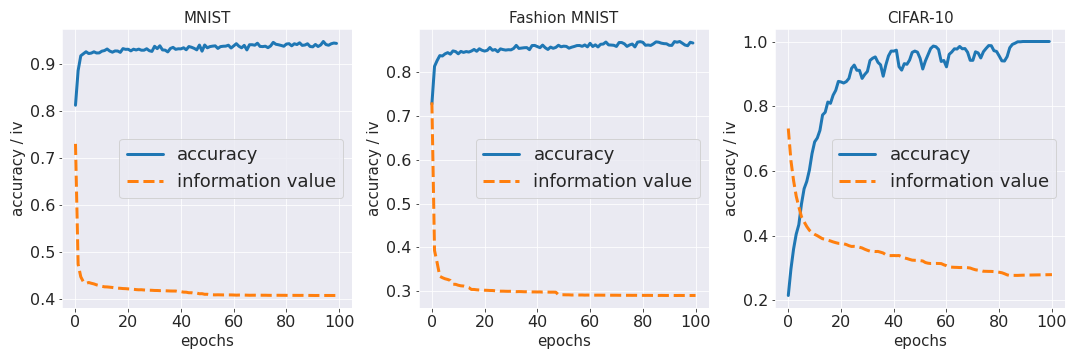
\includegraphics[scale=0.3]{paper/iv.png}
\captionof{figure}{Information Transfer Rate vs Accuracy}
\label{fig:iv.png}
\end{figure}


% \begin{minipage}{.4\textwidth}
% Figure \ref{fig:iv.png} shows that over time, the number of features picked by the network saturates. On close observation, the saturation point of the $itr_{network}$ metric is similar to the saturation point of the accuracy function. MNIST and Fashion MNIST datasets are relatively easy datasets compared to CIFAR-10 and the saturation point of the metric can be used as an early-stopping criterion. In CIFAR-10, the metric changes over time and so does the accuracy and hence it does not meet the early exit criterion.
% \end{minipage}
% \begin{minipage}{.5\textwidth}
%     \centering
%     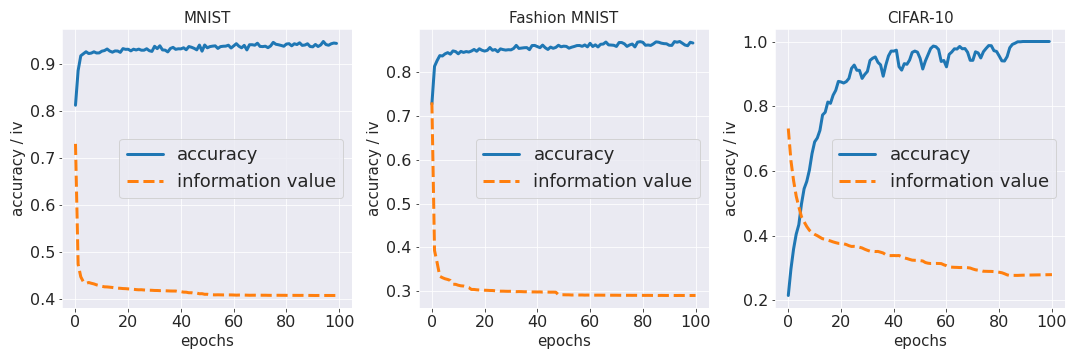
\includegraphics[scale=0.25]{paper/iv.png}
%     \captionof{figure}{Information Transfer Rate vs Accuracy}
%     \label{fig:iv.png}
% \end{minipage}

\subsubsection{Pruning}
\label{sec:Pruning}
To address the issue of an exponential increase in trainable parameters due to the merge operation in GSC, differentiable short circuit's weighted connection gates are used to selectively prune redundant nodes by removing connections.  If the current input is not important to the task, we define a binary function $f_{binary}$ whose output, when 0, the current input information shall not be passed on to the next layer. The input to the binary function ranges between 0 and 1. The probability of obtaining 0 or 1 for the binary function can be computed by,
\begin{equation}
\label{eq:ffn_math_representation}
\begin{aligned}
   P(f_{binary(x)}=1) &=x&\\
   P(f_{binary(x)}=0) &=1-P(f_{binary(x)}=1)&\\   
\end{aligned}
\end{equation}
However, the binary connection gate function is not differentiable and breaks backpropagation. There are generally two solutions. The first is to REINFORCE algorithms \cite{Williams1992SimpleSG} and considering its applications, it is computationally expensive and the reward is difficult to design to approximate the gradients. In recent times, few gradient estimators are proposed and among them, the Straight through gradient estimator \cite{Bengio2013EstimatingOP} is found to be useful due to its reduced computational complexity. The function approximates the step function by the identity when computing gradients during the backward pass:
\begin{equation}
\frac{\partial{f_{binaray}(x)}}{\partial x}=1
\end{equation}
With the implementation of a straight-through estimator, the model parameters can now be trained to optimize the use of connection weights $\hat{C}$ with standard backpropagation without defining any additional supervision or reward signal. This assures that the computation complexity does not increase.

\noindent\begin{minipage}{.5\textwidth}
   \centering
   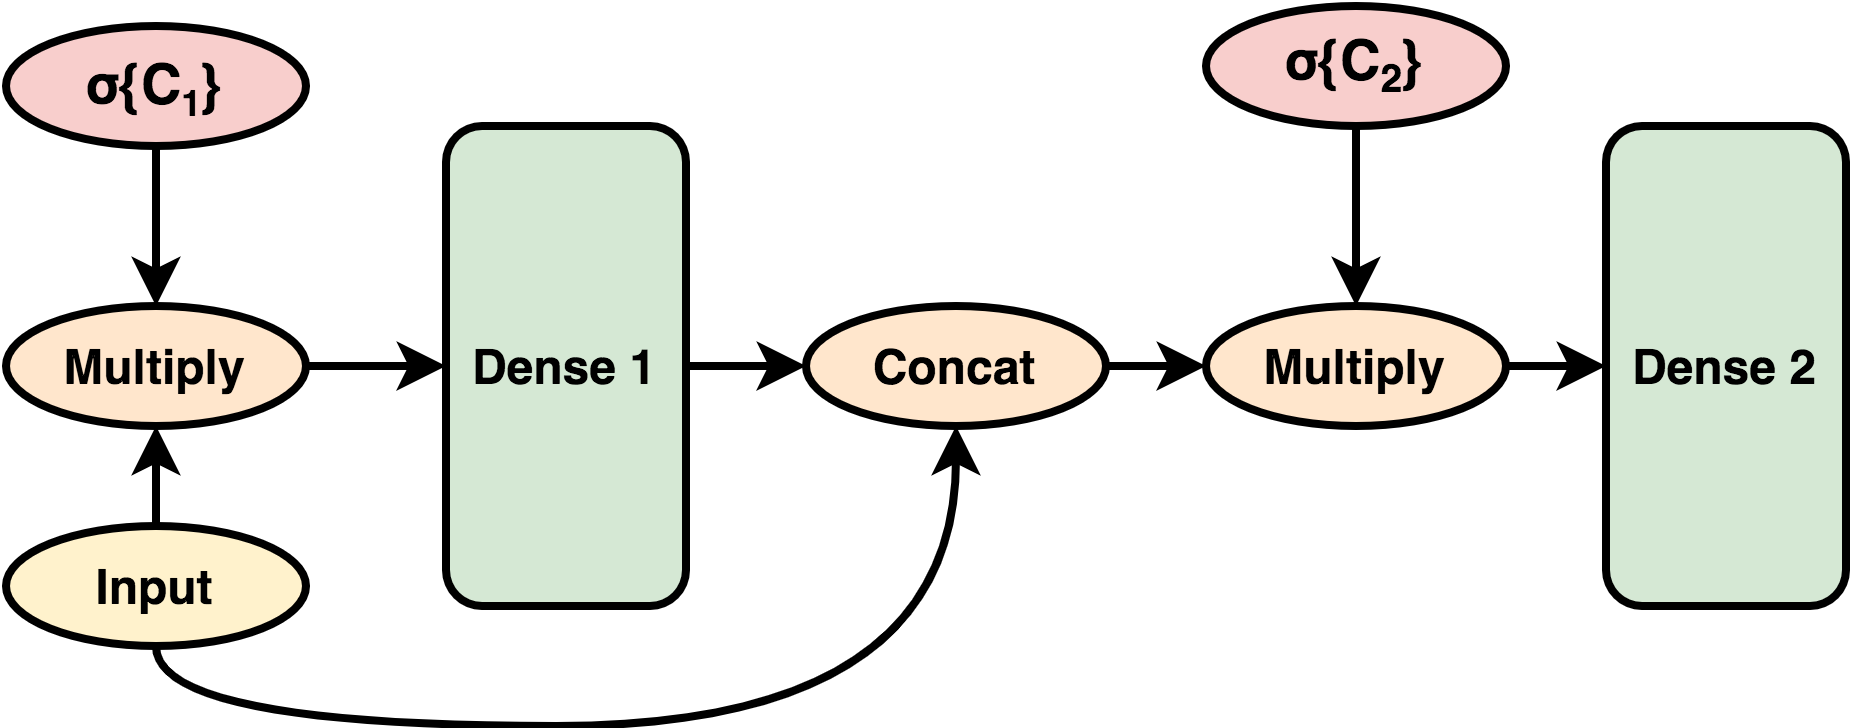
\includegraphics[scale=0.1]{paper/Pruning1.png}
   \captionof{figure}{2-Layer DSC architecture}
  \label{fig:pruning1.png}
\end{minipage}
\begin{minipage}{.4\textwidth}
\centering
   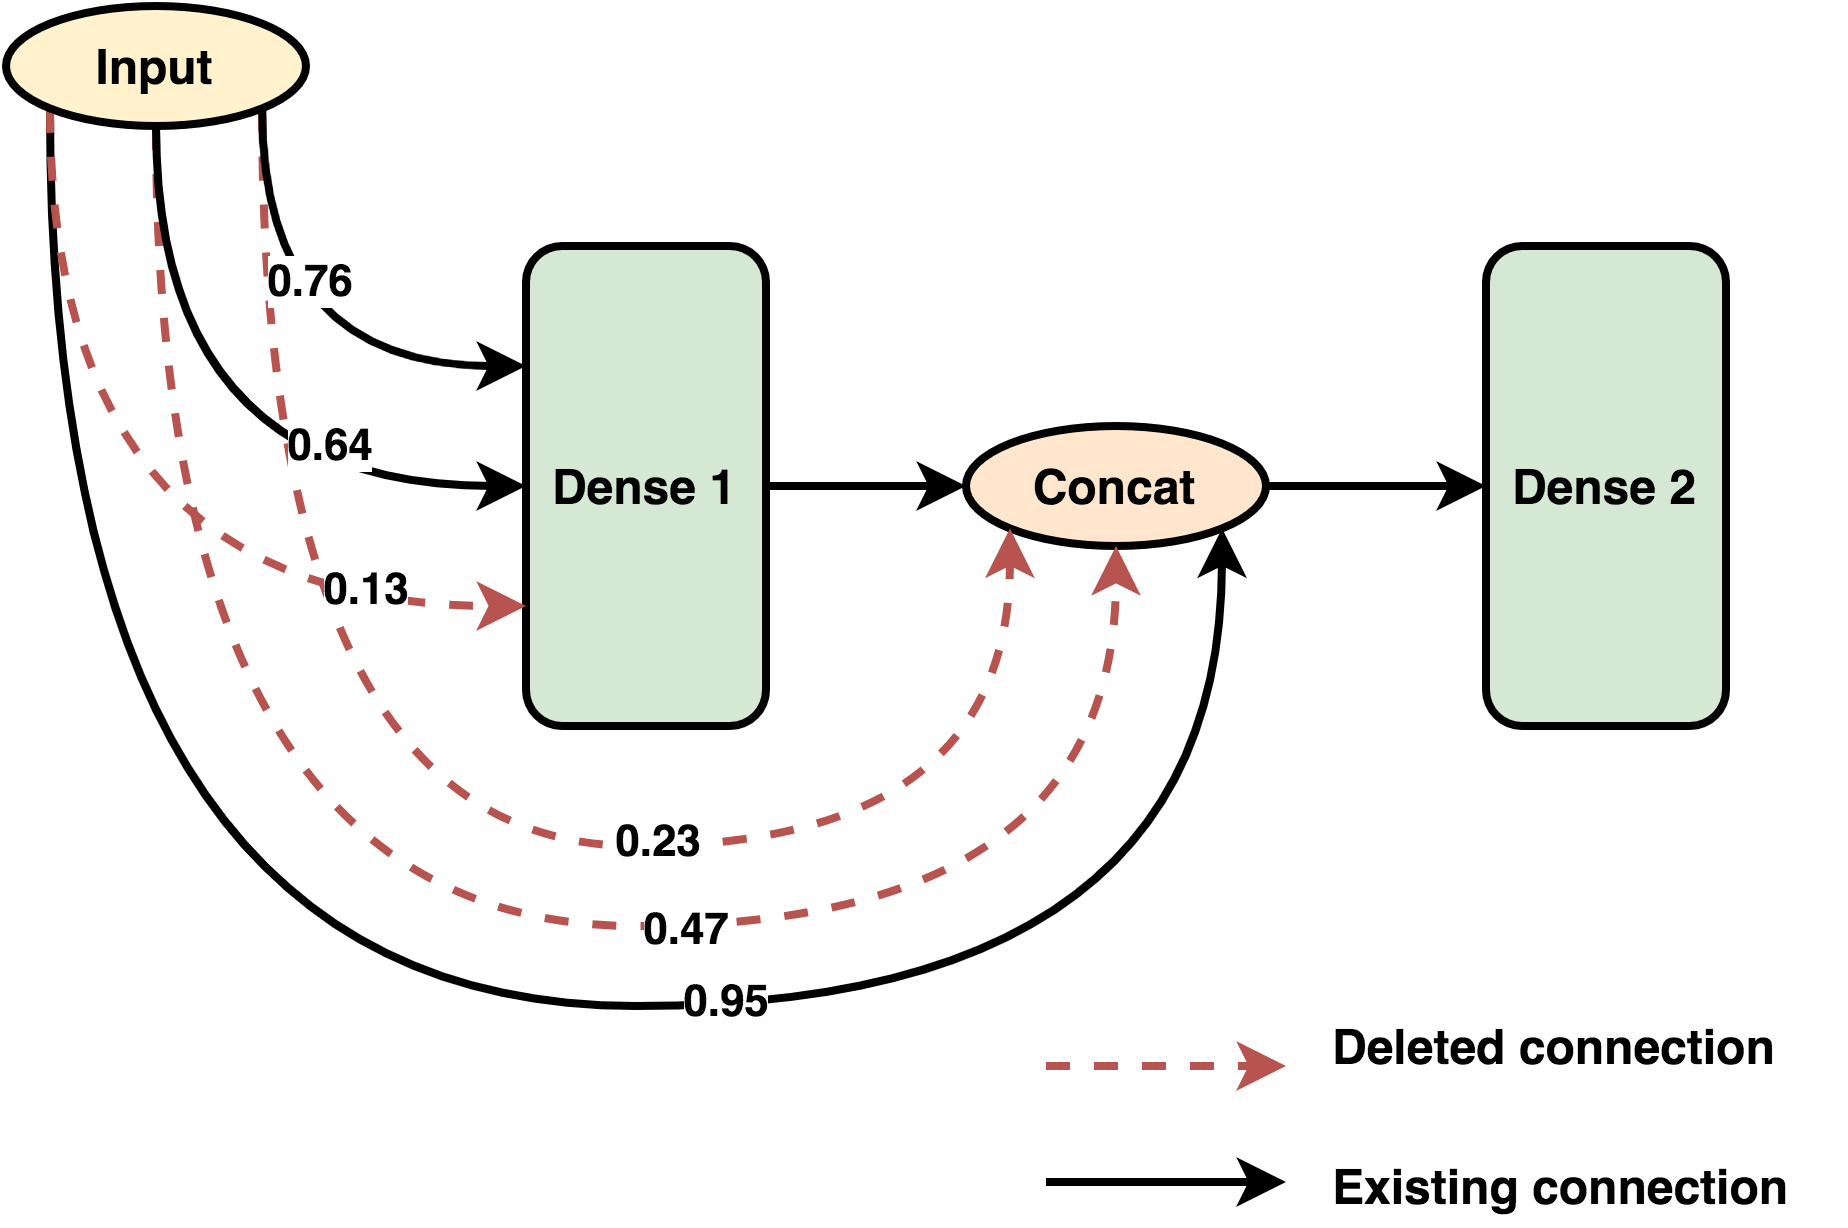
\includegraphics[scale=0.09]{paper/Pruning2.png}
   \captionof{figure}{Pruned connections}
\label{fig:pruning2.png}
\end{minipage}

Figure \ref{fig:pruning1.png} shows a 2-layered DSC network with all the necessary operations (concat, multiply . . .) including skip connection from input to the dense layer. To the right, Figure \ref{fig:pruning2.png} shows connections from input to dense layers. The floating-point number represents the value of  $\sigma(\hat{C_{i}})$. Based on the binary gate, a threshold of 0.5 is used, and the ones having values less than 0.5 have a different representation to mark the connection to be pruned.

\noindent\begin{minipage}{.5\textwidth}
  \begin{algorithm}[H]
  
\SetAlgoLined
\KwResult{Prune the network based on binary mask}

\For{layer in network layers;}{
\textit{prune nodes}\textsuperscript{(i)} 	\leftarrow\textit{compute nodes to prune(layer)}

}

i \leftarrow \textit{Number of layers}


 \While{i $<$ 0}{
  \textit{layer} \gets\ \textit{prune}\textit{(layer}\textsuperscript{(i)}, \textit{prune nodes}\textsuperscript{(i)}\textit{)}\

}
 
 \Procedure {prune}{$layer, nodes$}
    \State $layer.weight\gets\ layer.weight[:,nodes]}$ 
    \State $layer.bias\gets\ {layer.bias[:,nodes]} $ 
    \State $layer.connections \gets\ layer.connections[nodes]$ 
    \State \textbf{return} $layer$ 
\EndProcedure
 
 \caption{Dependency based pruning}
\end{algorithm}

\end{minipage}
\begin{minipage}{.4\textwidth}
In the first for loop we iterate the network layer wise, build dependency graph, collect the nodes falling under prune criteria and store it in $prune$ $nodes$. We then iterate backwards to change layer weights, biases and connection weights based on $prune$ $nodes$. 
\par% 
\bigskip
The $prune$ function takes a layer and the corresponding prune indices and calculates new layer dimensions. It also clones the layer weights, layer bias, connection weights and extracts appropriate indices to match the layer dimensions of the new layer. Finally the new set of parameters are assigned to layer created in the previous step.
\end{minipage}

\par
\bigskip

\par
\bigskip


\section{Experiments}
\label{sec:experiments}

For the experiments, we prefer to use MNIST, Fashion-MNIST and CIFAR-10 datasets. These datasets are chosen based on the complexity in the class patterns. We run hyperparmeter tuning \footnote{Combinations of Batch size[32,64,256], learning rate[1e-1, 1e-2, 1e-3], learning rate decay[False, 1] and regularization coefficients[1, 1e-1, 1e-2, 1e-3] are tried against 5 splits of training, validation and test datasets. Tables \ref{tab:100p_data_config} and \ref{tab:10p_data_config} describes the splits across datasets in detail. } across CV-5 for each of our experiments. This ensures that each network is tuned respectively to get the best performance. We define two sets of data and network architectures,
\begin{itemize}
\item 100p Data (Table \ref{tab:100p_data_config}) - Model is trained on all of the available training data and is tested against the standard set containing 10,000 samples. This is a standard set to determine the optimum performance of the networks.
\item 10p Data (Table \ref{tab:10p_data_config}) - Model is trained on 10\% of the available training data and is tested against a large set i.e, 10,000 samples. We use this experiment to test our hypothesis - GSC and DSC neural architectures enable models to develop deep constructs compared to the standard architecture.
\item 100p Params (Table \ref{tab:100p_param_config}) - This set defines a standard neural architecture for the model design, where the number layers and the number of nodes in the layer are kept constant across architectures. However, we see a 30\% rise in trainable parameters for GSC and DSC architectures compared to the standard architecture. This is due to the merge operation on skip connections.
\item 10p Params (Table \ref{tab:10p_param_config}) - Here, 10\% of the original DSC's architecture is used. Based on the resulting trainable parameters, the other networks are designed to match this. Though the architectures are different, the number of trainable parameters are kept constant across the networks in this set. It is designed as a counter to the argument - The difference in the performance of the networks is solely dependent on the number of trainable parameters.
\end{itemize}


\begin{tabular}{cc}
    \begin{minipage}{.5\linewidth}
\centering
\begin{tabular}{@{}llll@{}}
\toprule
\textbf{Dataset} & \textbf{Train} & \textbf{Valid} & \textbf{Test} \\ \midrule
MNIST            & 50000          & 10000          & 10000         \\
Fashion MNIST    & 50000          & 10000          & 10000         \\
CIFAR            & 40000          & 10000          & 10000         \\ \bottomrule
\end{tabular}
   \captionof{table}{100p Data sample split}
\label{tab:100p_data_config}
    \end{minipage} &
    \begin{minipage}{.5\linewidth}
    \centering
    \begin{tabular}{@{}llll@{}}
\toprule
\textbf{Dataset} & \textbf{Train} & \textbf{Valid} & \textbf{Test} \\ \midrule
MNIST            & 5000          & 1000          & 10000         \\
Fashion MNIST    & 5000          & 1000          & 10000         \\
CIFAR            & 4000          & 1000          & 10000         \\ \bottomrule
\end{tabular}
\captionof{table}{10p Data sample split}
\label{tab:10p_data_config}
    \end{minipage} 
\end{tabular}


\begin{tabular}{cc}
    \begin{minipage}{.5\linewidth}
\centering
\begin{tabular}{@{}llll@{}}
\toprule
\textbf{Model} & \textbf{MNIST} & \textbf{Fashion MNIST} & \textbf{CIFAR-10} \\ \midrule
FFN            & 83550          & 83550                  & 162810            \\
GSC            & 122750         & 122750                 & 224250            \\
DSC            & 124418         & 124418                 & 226448            \\ \bottomrule
\end{tabular}
   \captionof{table}{100p Model Parameters}
\label{tab:100p_param_config}
    \end{minipage} &
    \begin{minipage}{.5\linewidth}
    \centering
    \begin{tabular}{@{}llll@{}}
\toprule
\textbf{Model} & \textbf{MNIST} & \textbf{Fashion MNIST} & \textbf{CIFAR-10} \\ \midrule
FFN            & 32425          & 32425                  & 31215             \\
GSC            & 15800          & 15800                  & 25775             \\
DSC            & 17378          & 17378                  & 27838             \\ \bottomrule
\end{tabular}
\captionof{table}{10p Model Parameters}
\label{tab:10p_param_config}
    \end{minipage} 
\end{tabular}


\subsection{100p Data - Large Training Set, Large Test Set}

Results show that DSC achieves the best performance across different datasets compared to standard and GSC architectures. The difference in performance is noticeably higher in CIFAR-10 due to its increased pattern complexity. Our proposed architecture achieves better accuracy in fewer iterations (~5000 iterations less) compared to standard architecture. When the 10p model is used, the accuracy does drop but is relatively better than the standard network.

\begin{figure}[h!]
\centering
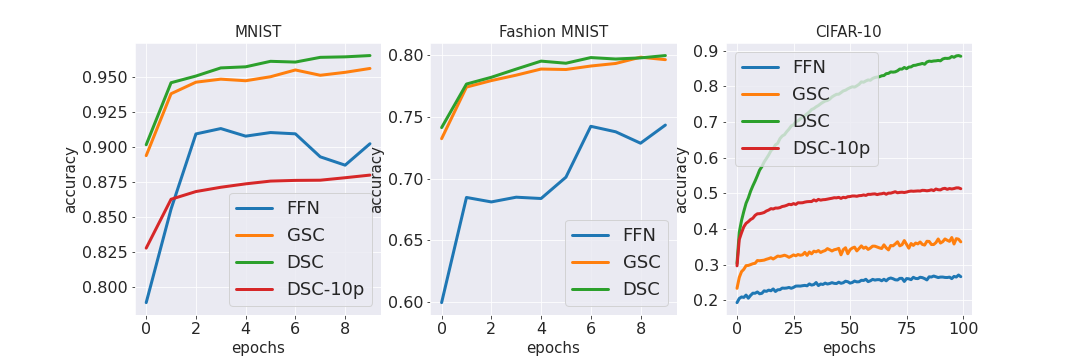
\includegraphics[scale=0.3]{paper/100p_runs.png}
\caption{100p Train comparison}
\label{fig:infotransfer}
\end{figure}

\begin{table}[H]
\centering
\begin{tabular}{llllll}
\hline
\multirow{2}{*}{\textbf{Model}}   & \multirow{2}{*}{\textbf{Parameter}} & \multirow{2}{*}{\textbf{Dataset}} & \multicolumn{2}{c}{\textbf{Train}}                & \multicolumn{1}{c}{\textbf{Test}} \\ \cline{4-6} 
                                  &                                     &                                   & \textbf{Accuracy @ Steps} & \textbf{Loss @ Steps} & \textbf{Accuracy}                 \\ \cline{1-3}
\multirow{3}{*}{Linear FFN}       & \multirow{3}{*}{83550}          & MNIST                    & 0.90 @ 7000          & 0.02 @ 7000          & 0.91                     \\
                                  &                                 & FashionMNIST             & 0.74 @ 7000          & 0.05 @ 7000          & 0.74                     \\
                                  &                                 & CIFAR-10                 & 0.27 @ 7000          & 1.87 @ 7000          & 0.20                     \\
                                  &                                 &                          &                      &                      &                          \\
\multirow{3}{*}{GSC}              & \multirow{3}{*}{122750}         & MNIST                    & 0.93 @ 1400          & 0.0113 @1400         & 0.93                     \\
                                  &                                 & FashionMNIST             & 0.72 @ 700           & 0.0481 @ 700         & 0.79                     \\
                                  &                                 & CIFAR-10                 & 0.28 @ 2100          & 2.53 @ 7000          & 0.29                     \\
                                  &                                 &                          &                      &                      &                          \\
\textbf{DSC}                      & \textbf{124418}                 & \textbf{MNIST}           & \textbf{0.95 @ 1400} & \textbf{0.01 @ 1400} & \textbf{0.96}            \\
\textbf{}                         & \textbf{}                       & \textbf{FashionMNIST}    & \textbf{0.74 @ 700}  & \textbf{0.05 @ 700}  & \textbf{0.79}            \\
\textbf{}                         & \textbf{}                       & \textbf{CIFAR-10}        & \textbf{0.3 @ 700}   & \textbf{2.1 @ 700}   & \textbf{0.40}            \\
                                  &                                 &                          &                      &                      &                          \\
\multirow{3}{*}{\textbf{DSC-10p}} & \multirow{3}{*}{\textbf{17378}} & \textbf{MNIST}           & \textbf{0.89 @ 2800} & \textbf{0.02 @ 2100} & \textbf{0.89}            \\
                                  &                                 & \textbf{FashionMNIST}    & \textbf{0.71 @ 700}  & \textbf{0.07 @ 700}  & \textbf{0.74}            \\
                                  &                                 & \textbf{CIFAR-10}        & \textbf{0.29 @ 700}  & \textbf{2.2 @ 700}   & \textbf{0.38}            \\ \cmidrule(l){3-6} 
\end{tabular}
\caption{100\% Data Results}
\label{tab:100p_data_table}
\end{table}


\subsection{10p Data - Minimal Training Set, Large Test Set}
\begin{figure}[h!]
\centering
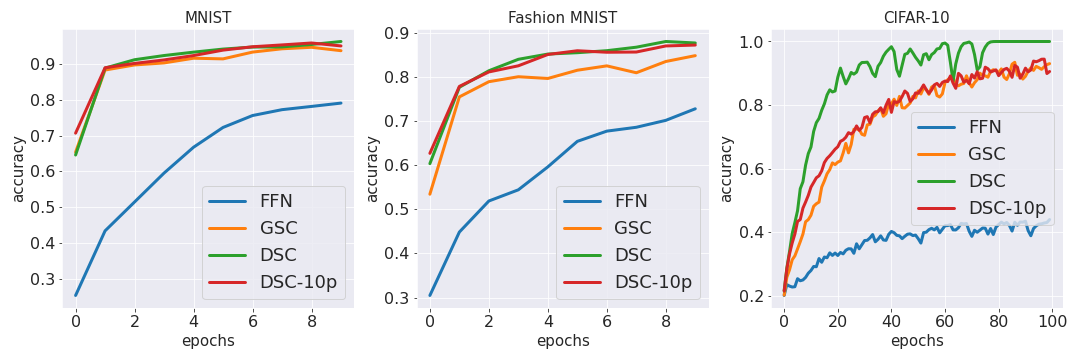
\includegraphics[scale=0.3]{paper/10p_runs.png}
\caption{10p Train comparison}
\label{fig:10p_runs}
\end{figure}

% Please add the following required packages to your document preamble:
% \usepackage{multirow}
\begin{table}[H]
\centering
\begin{tabular}{llllll}
\hline
\multirow{2}{*}{\textbf{Model}}   & \multirow{2}{*}{\textbf{Parameter}} & \multirow{2}{*}{\textbf{Dataset}} & \multicolumn{2}{c}{\textbf{Train}}                & \multicolumn{1}{c}{\textbf{Test}} \\ \cline{4-6} 
                                  &                                     &                                   & \textbf{Accuracy @ Steps} & \textbf{Loss @ Steps} & \textbf{Accuracy}                 \\ \cline{1-3}
\multirow{3}{*}{Linear FFN}       & \multirow{3}{*}{83550}              & MNIST                             & 0.79 @ 7000               & 0.70 @ 7000           & 0.74                              \\
                                  &                                     & FashionMNIST                      & 0.72 @ 7000               & 0.70 @ 7000           & 0.7                               \\
                                  &                                     & CIFAR-10                          & 0.44 @ 7000               & 1.45 @ 7000           & 0.22                              \\
                                  &                                     &                                   &                           &                       &                                   \\
\multirow{3}{*}{GSC}              & \multirow{3}{*}{122750}             & MNIST                             & 0.79 @ 2100               & 0.69 @ 2100           & 0.85                              \\
                                  &                                     & FashionMNIST                      & 0.72 @ 2100               & 0.70 @ 2100           & 0.76                              \\
                                  &                                     & CIFAR-10                          & 0.44 @ 700                & 2.46 @ 700            & 0.28                              \\
                                  &                                     &                                   &                           &                       &                                   \\
\textbf{DSC}                      & \textbf{124418}                     & \textbf{MNIST}                    & \textbf{0.88 @ 1400}      & \textbf{2.13 @ 1400}  & \textbf{0.89}                     \\
\textbf{}                         & \textbf{}                           & \textbf{FashionMNIST}             & \textbf{0.77 @ 1400}      & \textbf{1.91 @ 1400}  & \textbf{0.79}                     \\
\textbf{}                         & \textbf{}                           & \textbf{CIFAR-10}                 & \textbf{0.64 @ 700}       & \textbf{1.05 @ 700}   & \textbf{0.33}                     \\
                                  &                                     &                                   &                           &                       &                                   \\
\multirow{3}{*}{\textbf{DSC-10p}} & \multirow{3}{*}{\textbf{17378}}     & \textbf{MNIST}                    & \textbf{0.75 @ 700}       & \textbf{1.56 @ 700}   & \textbf{0.87}                     \\
                                  &                                     & \textbf{FashionMNIST}             & \textbf{0.77 @ 1400}      & \textbf{1.51 @ 1400}  & \textbf{0.77}                     \\
                                  &                                     & \textbf{CIFAR-10}                 & \textbf{0.43 @ 700}       & \textbf{1.6 @ 700}    & \textbf{0.26}                     \\ \cline{3-6} 
\end{tabular}
\caption{10\% Data Results}
\label{tab:10p_data_table}
\end{table}

This set tests the generalization of the networks. Figure \ref{fig:10p_runs} shows the performance of DSC against standard architecture across different datasets. As the number of training samples is limited to 10\% of the original data and a large test set it adopted, we monitor whether the network has an issue of overfitting. This is not the case with our proposed architecture. Table \ref{tab:10p_data_table}'s Test accuracy of DSC establishes that our proposed architecture has reduced overfit compared to others. There exists a noticeable drop in the performance of standard architecture in test metrics when compared to 100p data. The same is not observed in the DSC, as the 10p data model follows 100p data more closely.

\subsection{Understanding connection weights ($\hat{C}$)}
\label{subsec:understanding_connection_weights}
To comprehend the nature of gated connections, we create thresholded heatmaps of the weights. This is possible since connection weight is a function of $\sigma$ and skip connections from input to every other layer is considered. Figure \ref{fig:mnist_vis} and \ref{fig:fashion_mnist_vis} is a visual representation of connection weights from input to the other three layers defined in section \ref{sec:dsc} for MNIST and Fashion MNIST respectively. The borders of the input do not contain any valuable information and the network learns to discard these connections over time. The model learns to drop common features among different classes and this reduces class ambiguity and thereby increasing the confidence score of a class. The mean utilization of inputs represents the commonly used pixels across different classes and layers with high importance.

\begin{figure}[H]
\centering
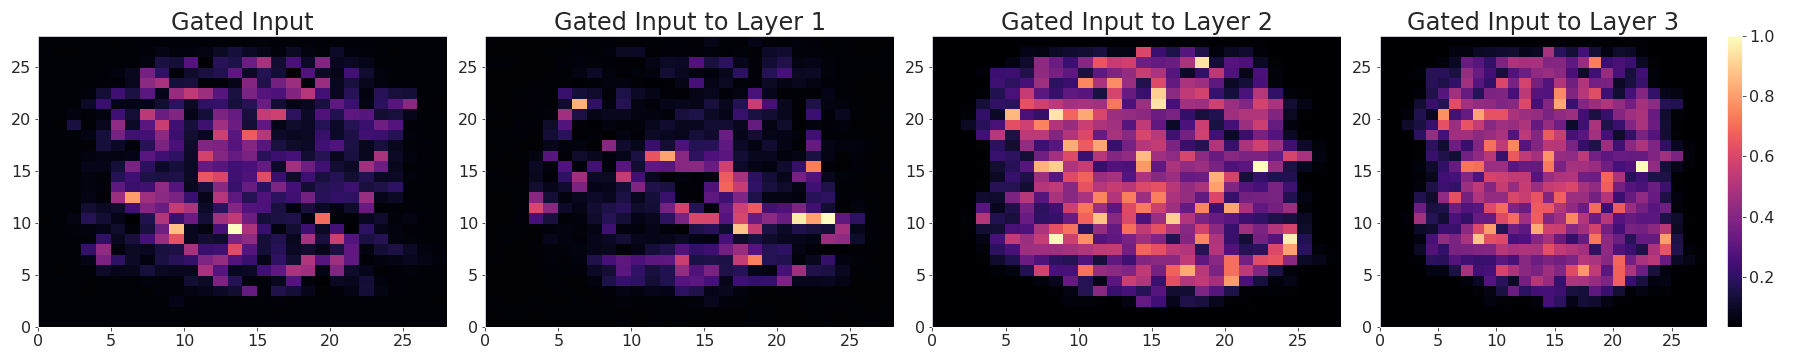
\includegraphics[scale=0.2]{paper/mnist_vis.png}
\captionof{figure}{MNIST Dataset}
\label{fig:mnist_vis}
\end{figure}

\begin{figure}[H]
\centering
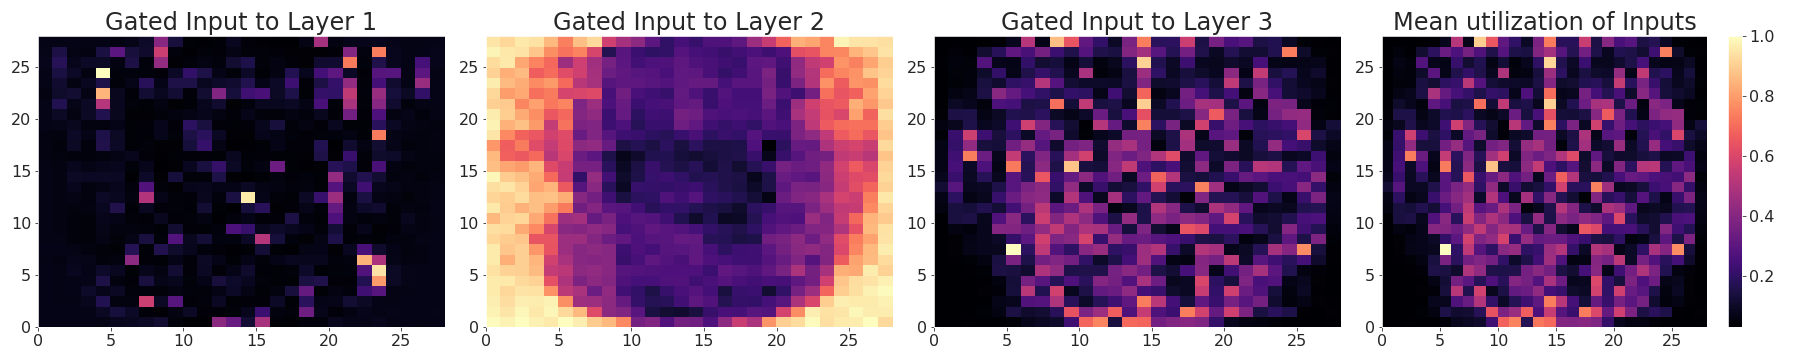
\includegraphics[scale=0.2]{paper/fashionmnist_vis.png}
\captionof{figure}{Fashion MNIST Dataset}
\label{fig:fashion_mnist_vis}
\end{figure}

\section{Conclusion}

Our work establishes the usefulness of global short circuits in improving the performance of the network by enabling the model to develop much deeper constructs compared to the standard architecture. We elucidate issues with global short circuit and propose differentiable short circuit as a solution. Differentiable short circuit builds upon GSC  with the goal of scalability. DSC architecture with the help of connection weights brings in innovations such as Information Transfer Rate, Pruning, Layer intake visualization among others. The architecture achieves the top accuracy in fewer iterations compared to standard architecture and GSC across all datasets. 

From our experiments, we can conclude that DSC reduces model overfit, achieves high training accuracy while still maintaining a relatively high test accuracy. As a counter to the argument - increase in the trainable parameters is solely responsible for the increase in performance, we design and test a relatively smaller network, where the number of trainable parameters is kept constant across architecture and the results show that DSC performs better compared to other architectures. The added benefit is that our proposed method is capable of learning at a much faster pace ($learning rate > 0.1$) and with the optimal use of learning rate scheduler, the method achieves local minima in fewer iterations compared to other models. With the help of pruning, we introduce the factor of sparsity which is aimed at reducing the number of trainable parameters while still maintaining a fairly high test accuracy. This can be highly beneficial on mobile and embedded devices where hardware resource is scarce.



\section{Future Work}

DSC on feed-forward neural networks stands as a testimony proving the proposed new architecture holds water. We see the surge in performance when skip connections along with differentiable units are introduced. 


\begin{itemize}
  \item We plan to implement a Differentiable Convolutional Neural Network, where a layer $N$ is fed filters from every layer before it i.e. ($N-1$ to $1$).
  \item Also, many interesting questions about how a Deep Neural Network captures representations can be answered from the process of Differentiable Network Pruning. To name a few,
  
  \begin{itemize}
    \item One can see if DSC has modelled any direct relationship between input layer and output layer(as DSC maintains connection weights between input and output. If the connection weights are close to 1, then all of input is being used by the output layer).
    \item Also, it is interesting to analyze which is the layer on which the output depends the most(i.e. output layer feeds off of every previous layer's output). 
  \end{itemize}
  \item Analyze the parameters to be cut down by pruning and dynamically control the pruning percentage based on required accuracy levels or training times etc.
\end{itemize}


\bibliographystyle{unsrt}  
\bibliography{references}

\comment{
As the network gets deep, it is difficult to train and the use of residual learning in the form of short-circuit connections eases the process of training.

 In order to find the right connections, the  connection is represented as a differentiable function and is optimized using $\frac{\partial loss}{\partial connection}$

The binary gate allows us to apply a threshold and distinguish the connection based on the imporatance.
}

\end{document}